\documentclass[12pt]{article}
\usepackage{ctex}
\usepackage[english]{babel}
\usepackage{blindtext}
\usepackage{nameref}
\usepackage{fancyhdr}
\usepackage{amsmath,amssymb,amsthm}
\usepackage{graphicx,float}
\usepackage{physics}
\usepackage{pgfplots}
\usepackage[a4paper, total={6in, 9in}]{geometry}

\graphicspath{{../image/}}

\pagestyle{fancy}
\fancyhf{}
\fancyhf[HL]{微分幾何1:向量與導數}
\fancyhf[CF]{\thepage}

\newcommand{\innerprod}[2]{\langle{#1},{#2}\rangle}
\newcommand{\id}{\mathtt{id}}

\newtheorem{definition}{定義}
\newtheorem*{theorem}{定理}
\newtheorem*{corollary}{衍理}
\newtheorem*{lemma}{引理}
\newtheorem*{proposition}{命題}
\newtheorem*{remark}{小記}
\newtheorem*{claim}{主張}
\newtheorem*{example}{示例}
\newtheorem*{axiom}{公設}
\newtheorem*{exercise}{即時練習}
\renewenvironment*{proof}{\textit{證明.}}{\hfill$\qed$}

\newenvironment*{sol}{\par \textbf{解}.}{\hfill$\blacksquare$}

\begin{document}
    References: Introduction to Real Analysis (Bartle \& Sherbert), Thomas Calculus 12th Edition
    \section*{向量}

    向量屬於一種特殊的矩陣,通常用以表達\textbf{多維坐標}。

    \begin{definition}[向量]
        一個\textbf{$n$-維向量}包含$n$個元素,可視之爲\textbf{$n$-維空間}中的坐標,同時代表從原點指向該坐標的箭頭。
    \end{definition}
    
    爲方便描述,記$V_S$為帶有$S$域的元素的向量集合。

    \begin{definition}[向量加法]
        在向量集合$V_S$中,若$\vec{x}=(x_i)_i=(x_1,x_2,\dots),\vec{y}=(y_i)_i=(y_1,y_2,\dots)\in V_S$,則$$\vec{x}+\vec{y}:=(x_1+y_1,x_2+y_2,\dots)=(x_i+y_i)_i$$
    \end{definition}

    \begin{exercise}
        求以下向量和:\begin{enumerate}
            \item $(1,2)+(3,4)$;
            \item $(1,2,3,4)+(1,3,4,5)$;
            \item $(1,-1,-1,1,1,1)+(-1,1,1,-1,-1,-1)$.
        \end{enumerate}
    \end{exercise}

    \begin{definition}[標量乘法]
        在向量集合$V_S$中,若$\vec{x}=(x_i)_i=(x_1,x_2,\dots)\in V_S$,$\alpha \in S$,則$$\alpha \vec{x}:=(\alpha x_1,\alpha x_2,\dots)=(\alpha x_i)_i$$
    \end{definition}

    \begin{exercise}
        求以下標量積:\begin{enumerate}
            \item $3(1,2)$;
            \item $-7(1,3,4,5)$;
            \item $-1(-1,1,1,-1,-1,-1)$.
        \end{enumerate}
    \end{exercise}

    \begin{definition}[向量的量值]
        對於任意向量$\vec{v}$,其量值定義爲$|\vec{v}|$,代表其長度。
    \end{definition}
    \section*{向量空間}

    \begin{definition}[向量空間]
        設$V_S$為向量集合,且$\vec{x},\vec{y},\vec{z}\in V_S$, $\alpha, \beta \in S$。若$V_S$符合以下定理:\begin{itemize}
            \item 加法結合律:$(\vec{x}+\vec{y})+\vec{z}=\vec{x}+(\vec{y}+\vec{z})$。
            \item 加法交換律:$\vec{x}+\vec{y}=\vec{y}+\vec{z}$。
            \item 加法單位元:$\vec{0}\in V_S$使得$\vec{x}+\vec{0}=\vec{0}+\vec{x}=\vec{x}$。
            \item 加法逆:$\forall \vec{x}\in V_S$, 存在$\vec{y}\in V_S$使得$\vec{x}+\vec{y}=\vec{y}+\vec{x}=\vec{0}$。
            \item 標乘結合律:$\alpha(\beta \vec{x})=(\alpha\beta)\vec{x}$。
            \item 標乘單位元:$1\in S$使得$1\vec{x}=\vec{x}$。
            \item 分配律1:$\alpha(\vec{x}+\vec{y})=\alpha\vec{x}+\alpha\vec{y}$。
            \item 分配律2:$(\alpha+\beta)\vec{x}=\alpha\vec{x}+\beta\vec{x}$。
        \end{itemize}
    \end{definition}

    \begin{example}
        $\mathbb{R}$是一個向量空間。而且任何域也是向量空間。
    \end{example}

    \begin{example}
        在牛頓力學中討論力時,我們會以向量表示力的大小與方向。假設目前的討論僅限於平面(二維空間),並記施力點為原點$O$。
        \begin{figure}[H]
            \centering
            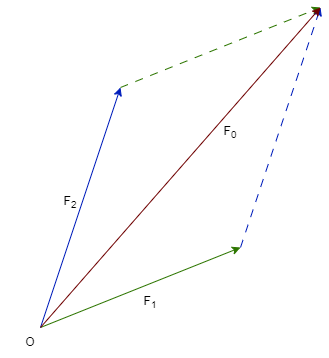
\includegraphics[scale=0.6]{Force.png}
        \end{figure}
        在上圖中可通過改變力量發生的先後次序來實現向量的平移,從而得出$$\vec{F_0}=\vec{F_1}+\vec{F_2}$$的關係式。
        又因二維向量可拆分爲水平向量及鉛垂向量兩個分量,故$$\vec{F_0}=(|\vec{F_1}|\cos{\theta}+|\vec{F_2}|\cos{\phi})\hat{i}+(|\vec{F_1}|\sin{\theta}+|\vec{F_2}|\sin{\phi})\hat{j}$$其中$\hat{i}$和$\hat{j}$分別代表水平單位向量及鉛垂單位向量。
    \end{example}

    欲考慮作功問題,我們定義以下計算方式

    \begin{definition}[點積/内積]
        兩向量$\vec{a},\vec{b}$的内積可定義爲$$\innerprod{\vec{a}}{\vec{b}}\equiv \vec{a}\cdot\vec{b}:=|\vec{a}||\vec{b}|\cos{\theta}$$其中$\theta$為$\vec{a},\vec{b}$之間的夾角。
    \end{definition}

    \begin{example}
        根據經典力學定義,作功方程爲$$W=\vec{F}\cdot\vec{s}$$其中$W$為作功純量,$\vec{F}$為施力向量,$\vec{s}$為位移向量。考慮内積定義,作功方程可寫成$$W=|\vec{F}||\vec{s}|\cos{\theta}$$其中$\theta$為向量之間的夾角。
    \end{example}

    \begin{theorem}[内積的性質]
        對於$\vec{a},\vec{b},\vec{c}$,\begin{enumerate}
            \item $\innerprod{0}{\vec{a}}=\innerprod{\vec{a}}{0}=0$;
            \item $\innerprod{\vec{a}}{\vec{a}}\geq 0$,$\innerprod{\vec{a}}{\vec{a}}=0$當且僅當$\vec{a}\equiv 0$;
            \item $\innerprod{\vec{a}}{x\vec{b}+z\vec{c}}=x\innerprod{\vec{a}}{\vec{b}}+z\innerprod{\vec{a}}{\vec{c}}$;
            \item 若$\vec{a},\vec{b}\in\mathbb{R}^n$,則$\innerprod{\vec{a}}{\vec{b}}=\innerprod{\vec{b}}{\vec{a}}$。
        \end{enumerate}
    \end{theorem}

    \begin{proposition}
        向量$\vec{a},\vec{b}$之間的夾角為$$\theta=\arccos{\frac{\vec{a}\cdot\vec{b}}{|\vec{a}||\vec{b}|}}$$
    \end{proposition}

    另外,若$\vec{a}$正交於$\vec{b}$(在$\mathbb{R}^2$為互相垂直),$\vec{a},\vec{c}$平行,則根據定義$$\vec{a}\cdot\vec{b}=|\vec{a}||\vec{b}|\cos{90^\circ}=0$$及$$\vec{a}\cdot\vec{c}=|\vec{a}||\vec{c}|\cos{0^\circ}=|\vec{a}||\vec{c}|$$
    因此$$|\vec{a}|=\sqrt{|\vec{a}|^2}=\sqrt{\innerprod{\vec{a}}{\vec{a}}}$$
    \begin{definition}[基與正交基與標準正交基]
        對於向量空間$V_S$,若$\{\vec{b_1},\vec{b_2},\dots,\vec{b_n}\}\subset V_S$為互不平行,即綫性獨立,同時對任意$\vec{v}\in V_S$,都存在$\alpha_1,\alpha_2,\dots,\alpha_n\in S$使得$$\vec{v}=\sum_{k=1}^{n}\alpha_k \vec{b_k}$$則稱$\{\vec{b_1},\vec{b_2},\dots,\vec{b_n}\}$為$V_S$的\textbf{基}。

        若$\{\vec{\beta_1},\vec{\beta_2},\dots,\vec{\beta_n}\}\subset V_S$為$V_S$的基而且對所有$i\neq j$,均有$$\innerprod{\vec{\beta_i}}{\vec{\beta_j}}=0$$則稱$\{\vec{\beta_1},\vec{\beta_2},\dots,\vec{\beta_n}\}$為$V_S$的\textbf{正交基}。

        若$\{\vec{\gamma_1},\vec{\gamma_2},\dots,\vec{\gamma_n}\}\subset V_S$為$V_S$的正交基而且對所有$i$,均有$$|\vec{\gamma_i}|=1$$則稱$\{\vec{\gamma_1},\vec{\gamma_2},\dots,\vec{\gamma_n}\}$為$V_S$的\textbf{標準正交基}。
    \end{definition}
    
    \begin{remark}
        對於任何向量空間,標準正交基的構成并非唯一。舉例$\mathbb{R}$作爲$\mathbb{R}$的向量空間,$1$和$-1$均可作爲$\mathbb{R}$的標準正交基;$\mathbb{R}^2$作爲$\mathbb{R}$的向量空間,則$$\{\begin{bmatrix}
            \cos{\theta}\\\sin{\theta}
        \end{bmatrix},\begin{bmatrix}
            -\sin{\theta}\\\cos{\theta}
        \end{bmatrix}:\theta\in\mathbb{R}\}$$均爲$\mathbb{R}^2$的標準正交基。
    \end{remark}

    對於有標準正交基的向量空間,我們的討論會比較簡單:

    \begin{theorem}
        設$V_S$為向量空間,$\{e_1,e_2,\dots,e_n\}$為$V_S$的標準正交基。若$v,u\in V_S$可寫作$v=\sum_{i=1}^{n}v_i e_i$及$u=\sum_{i=1}^{n}u_i e_i$,則$$\innerprod{u}{v}=\sum_{i=1}^{n}u_iv_i$$
    \end{theorem}

    \begin{proof}
        \begin{align*}
            \innerprod{u}{v}
            &=\innerprod{\sum_{i=1}^{n}u_i e_i}{\sum_{j=1}^{n}v_j e_j}
            =\sum_{i=1}^{n}u_i\innerprod{e_i}{\sum_{j=1}^{n}v_j e_j}
            =\sum_{i=1}^{n}\sum_{j=1}^{n}u_iv_j\innerprod{e_i}{e_j}\\
            &=\sum_{i=1}^{n}\sum_{j=1}^{n}u_iv_j\delta_{ij}
            =\sum_{\substack{
                i=j\\1\leq i,j\leq n
            }}u_iv_j
            =\sum_{i=1}^{n}u_iv_i
        \end{align*}
    \end{proof}

    \begin{corollary}
        設$V_S$為向量空間,$\{e_1,e_2,\dots,e_n\}$為$V_S$的標準正交基。若$v\in V_S$可寫作$v=\sum_{i=1}^{n}v_i e_i$,則$$|v|=\sqrt{\sum_{i=1}^{n}v_i^2}$$而且$$v_i=\innerprod{v}{e_i}$$
    \end{corollary}

    爲方便描述,接下來會稱$V_S$的標準正交基為$\mathcal{O}(V_S):= \{e_i\}_{i\in I}$,$I$為索引集。

    \begin{theorem}[餘弦定理]
        設$u,v\in V_S$,則$$|u-v|^2=|u|^2+|v|^2-2|u||v|\cos{\theta}$$其中$\theta$是$u,v$的夾角。
    \end{theorem}

    \begin{proof}
        設$u=\sum_{i\in I}u_ie_i, v=\sum_{i\in I}v_ie_i$,則\begin{align*}
            |u-v|^2&=\sum_{i\in I}(u_i-v_i)^2\\
            &=\sum_{i\in I}(u_i^2+v_i^2-2u_iv_i)\\
            &=\sum_{i\in I}u_i^2+\sum_{i\in I}v_i^2-2\sum_{i\in I}u_iv_i\\
            &=|u|^2+|v|^2-2\innerprod{u}{v}\\
            &=|u|^2+|v|^2-2|u||v|\cos{\theta}
        \end{align*}
    \end{proof}

    在三維空間中,存在外積:

    \begin{definition}[外積]
        假設$\{\hat{i},\hat{j},\hat{k}\}\subset \mathbb{R}^3$為$\mathbb{R}^3$的標準正交基,則定義$\times:\mathbb{R}^3\to\mathbb{R}^3$為$$\hat{i}\times \hat{j}=\hat{k},\hat{j}\times \hat{k}=\hat{i}, \hat{k}\times \hat{i}=\hat{j}$$
    \end{definition}

    外積的定義可考慮面積與體積的計算原理:考慮三個單位向量$\hat{i},\hat{j},\hat{k}$的乘積為體積及任意兩個向量的乘積為面積,基於$\hat{i}\times \hat{j}$為$ij$平面的面積單位,而面積乘以高等於體積,故$V(\hat{i},\hat{j},\hat{k})=(\hat{i}\times \hat{j})\cdot \hat{k}$為標量,使得$\hat{i}\times\hat{j}=\hat{k}$。

    因此,我們可定義

    \begin{definition}[面積與體積]
        設$u,v,w\in\mathbb{R}^3$,則\begin{align*}
            A(u,v)&:=|u\times v|=\left|\left|\begin{matrix}
                \hat{i}&\hat{j}&\hat{k}\\
                u_1&u_2&u_3\\
                v_1&v_2&v_3
            \end{matrix}\right|\right|\\
            V(u,v,w)&:=(u\times v)\cdot w=\left|\begin{matrix}
                u_1&u_2&u_3\\
                v_1&v_2&v_3\\
                w_1&w_2&w_3
            \end{matrix}\right|\\
        \end{align*}
    \end{definition}

    事實上,外積的計算無法以向量簡單作結。Kronecker就發現基本的向量無法解釋$i\times j=k$的情況(例如,爲何面積是向量而體積不是?),因此,他提出以\textbf{雙向量}(bi-vector)為$\hat{i},\hat{j},\hat{k}$下定義:

    \begin{definition}
        定義$\hat{i}=e_1e_2,\hat{j}=e_2e_3,\hat{k}=e_1e_3$,且$e_ie_j=-e_je_i$,$e_i^2=1$由此符合\begin{align*}
            \hat{i}\hat{j}&=e_1e_2e_2e_3=e_1e_3=\hat{k}\\
            \hat{j}\hat{k}&=e_2e_3e_1e_3=-e_2e_3e_3e_1=-e_2e_1=e_1e_2=\hat{i}\\
            \hat{k}\hat{i}&=e_1e_3e_1e_2=-e_3e_1e_1e_2=-e_3e_2=e_2e_3=\hat{j}
        \end{align*}
    \end{definition}

    上述定義可引申至對軸心的旋轉:$\hat{i}$為沿$z$軸逆時針旋轉90度;$\hat{j}$為沿$x$軸逆時針旋轉90度;$\hat{k}$為沿$y$軸逆時針旋轉90度。

    事實上,在更高維的空間裏,向量的外積有以下定義

    \begin{definition}
        設$u=(u_i)_{i\in I},v=(v_i)_{i\in I}$,則外積為$$u\wedge v =\begin{bmatrix}
            u_1v_1&u_1v_2&\cdots&u_1v_n\\
            u_2v_1&u_2v_2&\cdots&u_2v_n\\
            \vdots&\vdots&\ddots&\vdots\\
            u_n v_1&u_n v_2&\cdots&u_n v_n
        \end{bmatrix}$$
    \end{definition}

    \begin{theorem}
        設$u,v\in \mathbb{R}^n$,則平行四邊形面積爲$$A(u,v)=|u||v|\sin{\theta}$$其中$\theta$為$u$和$v$的夾角。因此$$|u\wedge v|=|u||v|\sin{\theta}$$
    \end{theorem}

    \begin{corollary}
        設$u,v\in \mathbb{R}^n$,則$$|u|^2|v|^2=\innerprod{u}{v}^2+|u\wedge v|^2$$
    \end{corollary}

    外積的應用并不廣汎,因爲在高維空間其實很難定義内外,因此我們通常更集中於内積的運算。其中對於互補空間的探索可謂是將内積運用至極緻。
    
    \begin{definition}[維度]
        若某向量空間$V$的標準正交基有$n$項綫性獨立元素,則稱$V$是一個$n$維空間。記$\dim{V}=n$。
    \end{definition}

    \begin{definition}[補空間]
        設$V \subset \mathbb{R}^n$同時$\dim{V}=k< n$。若存在$V^{\perp}\subset \mathbb{R}^n$使得\begin{enumerate}
            \item $\dim{V^{\perp}}=n-k$及;
            \item $\forall v\in V, \forall v^{\perp}\in V^{\perp}$使得$$\innerprod{v}{v^{\perp}}=0$$
        \end{enumerate}
        則稱$V^{\perp}$為$V$的補空間。
    \end{definition}

    因此,$V^{\perp}$通常被定義爲$$V^{\perp}:=\{w\in\mathbb{R}^n:\innerprod{w}{v}=0, \forall v\in V\}$$

    \begin{example}
        在$\mathbb{R}^2$上,下列情況均為互補空間:\begin{enumerate}
            \item $\mathbf{X}:=\{(x,0)\in\mathbb{R}^2\}$及$\mathbf{Y}:=\{(0,y)\in\mathbb{R}^2\}$;
            \item $\forall u,v \in\mathbb{R}^2$,若$\innerprod{u}{v}=0$,則$\mathbf{U}:=\{ku:k\in\mathbb{R}\}$及$\mathbf{V}:=\{hv:h\in\mathbb{R}\}$為互補空間。
        \end{enumerate}
    \end{example}

    考慮$u,v\in\mathbb{R}^n$使得$u\wedge v\neq 0$,令$w:=u-\frac{\innerprod{u}{v}}{|v|^2}v$則$$\innerprod{u}{w}=0$$由此,我們可得以下命題:

    \begin{proposition}[正交化]
        設$u,v\in \mathbb{R}^n$且$u\in U\subset \mathbb{R}^n$,則$u-\frac{\innerprod{u}{v}}{|v|^2}v\in U^{\perp}$。
    \end{proposition}

    \begin{proof}
        留做習題。
    \end{proof}

    \begin{theorem}[格林-史密特正交化]
        若$B_V=\{b_1,b_2,\dots,b_n\}$為向量空間$V$的基,并且$b_i\wedge b_j\neq 0$。令$\{\beta_1,\beta_2,\dots,\beta_n\}$為另一基集使得$$\beta_n:=b_n-\sum_{k=1}^{n-1}\frac{\innerprod{\beta_k}{b_n}}{|\beta_k|^2}\beta_k$$則$\{\beta_1,\beta_2,\dots,\beta_n\}$為$V$的正交基。
    \end{theorem}

    \begin{proof}
        利用命題,可證明$\{\beta_1,\beta_2,\dots,\beta_n\}$為$V$的正交集;又因$\{\beta_1,\beta_2,\dots,\beta_n\}$的元素為$B_V$的綫性組合,$B_V$亦可寫成$\{\beta_1,\beta_2,\dots,\beta_n\}$的綫性組合,因此$\{\beta_1,\beta_2,\dots,\beta_n\}$為$V$的基。
    \end{proof}

    \begin{example}
        求以$\{(1,2,3),(1,3,5),(1,0,1)\}$為基的向量空間的一組標準正交基。

        \begin{align*}
            \beta_1'&=(1,0,1)\\
            \beta_1&=\frac{\beta_1'}{|\beta_1'|}=\frac{1}{\sqrt{2}}(1,0,1)\\
            \beta_2'&=(1,2,3)-\frac{4}{2}(1,0,1)\\
            &=(-1,2,1)\\
            \beta_2&=\frac{\beta_2'}{|\beta_2'|}=\frac{1}{\sqrt{6}}(-1,2,1)\\
            \beta_3'&=(1,3,5)-\frac{6}{2}(1,0,1)-\frac{10}{6}(-1,2,1)\\
            &=(-\frac{1}{3},-\frac{1}{3},\frac{1}{3})\\
            \beta_3&=\frac{\beta_3'}{|\beta_3'|}=\frac{1}{\sqrt{3}}(-1,-1,1)
        \end{align*}
        因此,$V$的其中一組標準正交基為$\{\frac{1}{\sqrt{2}}(1,0,1),\frac{1}{\sqrt{6}}(-1,2,1),\frac{1}{\sqrt{3}}(-1,-1,1)\}$
    \end{example}

    \section*{向量函數}

    向量函數顧名思義在於將函數從一個向量空間映射向另一個向量空間,其形式可以看成

    \begin{definition}[向量函數]
        給定$f:\mathbb{R}^m\to\mathbb{R}^n$,設$x=(x_1,x_2,\dots,x_m)\in\mathbb{R}^m$及$y=(y_1,y_2,\dots,y_n)\in\mathbb{R}^n$,若$$y=f(x)$$則對於所有$1\leq k\leq n$,存在獨特的$f_k:\mathbb{R}^m\to\mathbb{R}$使得$$y_k=f_k(x)$$
    \end{definition}

    \begin{example}
        以下爲向量函數的例子:\begin{enumerate}
            \item $f(x):=x^2+3x+1$;
            \item $f(x,y,z):=xy+xz+3y-2z$;
            \item $f(x):=(x,x^2,x^2+x)$;
            \item $f(x,y):=(x^2y,xy^2,x^3-y^3)$.
        \end{enumerate}
    \end{example}

    由於向量函數相較實函數有更多偏差發生,例如$$f(x,y):=(\frac{1}{x-y},x^2+y^2)$$并不能在$x=y$的情況下連續,因此我們又需要調出那個萬用的極限。

    \begin{definition}[向量函數的極限]
        設$y=f(x)$,其中$y\in\mathbb{R}^n$。若存在$y_0\in\mathbb{R}^n$使得對於任意$\epsilon>0$,都有$\delta>0$使得$|x-x_0|<\delta$時$|f(x)-y_0|<\epsilon$,則稱$y_0$為$f(x)$在$x_0$的極限,記$\displaystyle y_0=\lim_{x\to x_0}f(x)$。
    \end{definition}

    \begin{definition}[向量函數的連續性]
        若$f(x_0)=\displaystyle \lim_{x\to x_0}f(x)$,則稱$f$在$x_0$上連續。
    \end{definition}

    \section*{偏導數與全導數}

    此後的函數均預設為連續函數。

    \begin{definition}[偏導數]
        設$f:\mathbb{R}^m\to\mathbb{R}^n$,而$(x_1,x_2,\dots,x_m)\overset{f}{\mapsto}(y_1,y_2,\dots,y_n)$。若只求$f$對於單一變量$x_k$的變化,則$$\partialderivative{f}{x_k}=\lim_{h\to 0}\frac{f(x_1,x_2,\dots,x_k+h,\dots,x_n)-f(x_1,x_2,\dots,x_k,\dots,x_n)}{h}$$

        考慮$f=(f^1,f^2,\dots,f^n)$的記法,可將之寫成$$(\partialderivative{f^1}{x_k},\partialderivative{f^2}{x_k},\dots,\partialderivative{f^n}{x_k})$$
    \end{definition}

    \begin{remark}
        偏導數的記法通常以$\displaystyle\partialderivative{f}{x}$表示,也有寫$\partial_x f$或$f_x$簡便記之。
    \end{remark}

    \begin{example}
        求$f(x,y,z):=xyz$的所有偏導數。

        \begin{align*}
            \partial_x f&=\partial_x(x)yz+x\partial_x(y)z+xy\partial_x(z)=yz\\
            \partial_y f&=\partial_y(x)yz+x\partial_y(y)z+xy\partial_y(z)=xz\\
            \partial_z f&=\partial_z(x)yz+x\partial_z(y)z+xy\partial_z(z)=xy
        \end{align*}
    \end{example}

    \begin{example}
        求$f(x,y):=(x^2,xy,xy^2)$的所有偏導數。

        \begin{align*}
            \partial_x f&=(\partial_x(x^2),\partial_x(xy),\partial_x(xy^2))=(2x,y,y^2)\\
            \partial_y f&=(\partial_y(x^2),\partial_y(xy),\partial_y(xy^2))=(0,x,2xy)
        \end{align*}
    \end{example}

    \begin{definition}[全導數]
        設$f:\mathbb{R}^m\to\mathbb{R}^n$,而$(x_1,x_2,\dots,x_m)\overset{f}{\mapsto}(y_1,y_2,\dots,y_n)$。則$f$的全導數為$$df:=\sum_{k=1}^{n}\partial_{x_k}f dx_k=\begin{bmatrix}
            f_{x_1}&f_{x_2}&\cdots&f_{x_m}
        \end{bmatrix}d(x_1,x_2,\dots,x_m)$$
    \end{definition}

    \subsection*{情況一:$\mathbb{R}^3\to\mathbb{R}$}

    \begin{example}
        設$\vec{v}=(x,y,z)$並考慮$f(x,y,z)=xyz$,\begin{align*}
            df&=\sum_{k=1}^{3}\partial_{x_k}f dx_k\\
            &=\partial_x f dx + \partial_y f dy + \partial_z f dz\\
            &=yz dx+ xz dy + xy dz\\
            &=\begin{bmatrix}
                yz&xz&xy
            \end{bmatrix}\begin{bmatrix}
                dx\\dy\\dz
            \end{bmatrix}\\
            &=\innerproduct{\begin{bmatrix}
                f_x&f_y&f_z
            \end{bmatrix}}{d\vec{v}}
        \end{align*}
    \end{example}

    \subsection*{情況二:$\mathbb{R}\to\mathbb{R}^3$}

    \begin{example}
        考慮$\vec{f}(t)=(t,t^2,t^3)$,\begin{align*}
            d\vec{f}&=\sum_{k=1}^{3}\partial_{x_k}f dx_k\\
            &=\partial_x f dt\\
            &=(1,2t,3t^2)dt\\
            &=\innerproduct{\vec{f}_t}{dt}
        \end{align*}
    \end{example}

    \subsection*{情況三:$\mathbb{R}^3\to\mathbb{R}^3$}

    \begin{example}
        設$\vec{v}=(x,y,z)$並考慮$f(x,y,z)=(x+y^2+z^3, x^3+y+z^2, x^2+y^3+z)$,\begin{align*}
            df&=\sum_{k=1}^{3}\partial_{x_k}f dx_k\\
            &=\partial_x f dx + \partial_y f dy + \partial_z f dz\\
            &=(1,3x^2,2x) dx+ (2y,1,3y^2) dy + (3z^2,2z,1) dz\\
            &=\begin{bmatrix}
                1&2y&3z^2\\3x^2&1&2z\\2x&3y^2&1
            \end{bmatrix}\begin{bmatrix}
                dx\\dy\\dz
            \end{bmatrix}\\
            &=\innerproduct{\begin{bmatrix}
                \vec{f}_x&\vec{f}_y&\vec{f}_z
            \end{bmatrix}}{d\vec{v}}
        \end{align*}
    \end{example}

    \section*{方向導數}

    \section*{切面與法綫}

    \section*{二維極值與鞍點}
\end{document}